\section{Method}
\label{sec:method}

% --- from chapter3_problem_formulation.tex (intro + 3.3.1) and chapter3_integration.tex (intro) ---
Multi-person pose grouping is treated in this work as a stage that follows keypoint detection and is independent of the detector.
A bottom-up keypoint detector produces a set of two-dimensional keypoint detections for the whole image,
each carrying one of the seventeen COCO joint types~\citep{lin2014coco}.
The grouping stage partitions those detections into person skeletons without access to the image or to the detector's
internal representation (Figure~\ref{fig:pipeline}); the only quantities that cross the interface between the detector
and the grouping module are the keypoint coordinates, the visibility flags and the joint types.
The detector can therefore be replaced without changing or retraining the grouping network, and this separation is the
central design choice of the work.
It departs from architectures in which detection and grouping are learned together,
such as associative embedding~\citep{newell2017associative}, DEKR~\citep{geng2021dekr}
and ED-Pose~\citep{yang2023edpose},
whose grouping mechanism is tied to the features of the detector it was trained with.

\begin{figure*}[!t]
    \centering
    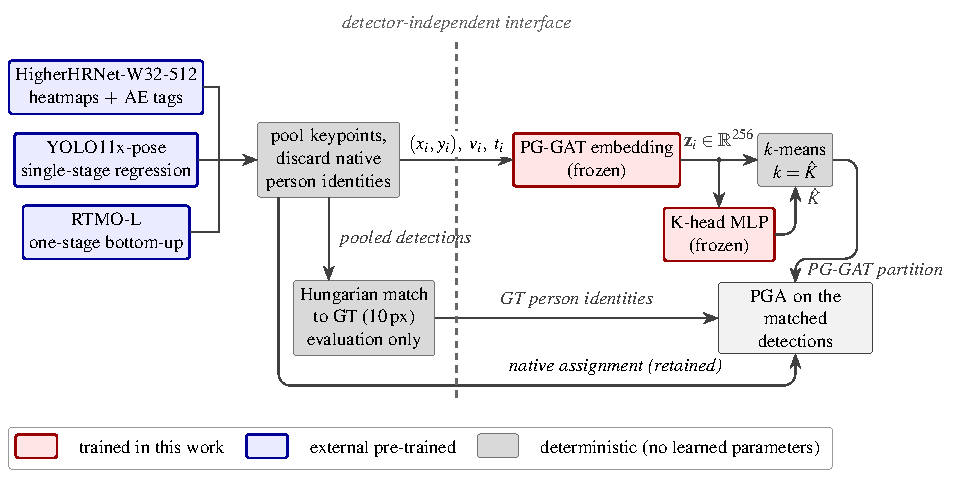
\includegraphics[width=\textwidth]{figures/e2e_interface.pdf}
    \caption{The detector-independent interface.
    Each detector produces a set of keypoint detections; its native person assignments are discarded,
    and only the keypoint coordinates, visibility flags and joint types cross the interface (dashed line).
    The frozen PG-GAT embeds the detections, the frozen K-head estimates the person count $\hat K$,
    and $k$-means produces the partition.
    Ground truth is used only for evaluation: detections are matched to the annotated keypoints,
    and both the PG-GAT partition and the detector's retained native assignment are scored on the matched set.}
    \label{fig:pipeline}
\end{figure*}

\subsection{Problem formulation}
\label{sec:method_problem}

% --- from chapter3_problem_formulation.tex 3.3.1 and 3.3.3 ---
For an image containing $K$ people, the detector produces $N$ keypoint detections, collected into the set
\begin{equation}
    \mathcal{X}
    = \bigl\{(\mathbf{p}_i, t_i, v_i)\bigr\}_{i=1}^{N},
    \label{eq:detections}
\end{equation}
where $\mathbf{p}_i \in [0,1]^2$ is the normalised image-plane position of detection $i$,
$t_i \in \mathcal{T} = \{1,\dots,T\}$ is its joint type with $T=17$ for COCO,
and $v_i$ is its visibility state.
The grouping task is to predict a labelling
\begin{equation}
    \hat{\mathbf{y}} \in \{1,\dots,K\}^{N},
    \label{eq:labelling}
\end{equation}
in which two detections share a label if and only if they belong to the same person.
Ground-truth assignments $\mathbf{y}^{\star}$ are available during training;
at inference the number of people $K$ is unknown and must be estimated from the detections themselves.

The problem is decomposed into three components.
An embedding network maps every detection to a vector $\mathbf{z}_i \in \mathbb{R}^{d}$ such that detections of the same
person lie close together and detections of different people lie apart.
A read-out recovers the person assignments from the embeddings, given $K$.
A person-count estimator supplies $K$ when no oracle value is available.
The embedding network carries the discriminative work, the read-out is deliberately kept simple,
and the count estimator is trained separately so that it cannot alter the embedding.

\subsection{Graph construction}
\label{sec:method_graph}

% --- from chapter3_problem_formulation.tex 3.3.2 and chapter3_dataset.tex (node features) ---
The detections of a single image form a graph $\mathcal{G} = (\mathcal{V}, \mathcal{E})$ with one node per detection,
$|\mathcal{V}| = N$.
The continuous node feature is
\begin{equation}
    \mathbf{x}_i
    =
    [\,x_{\text{norm}},\;
      y_{\text{norm}},\;
      v_{\text{norm}}\,]
    \in \mathbb{R}^{3},
    \label{eq:node_feature_no_depth}
\end{equation}
the image-plane position, normalised by the image size, and the visibility, scaled to $[0,1]$
(0.5 for an occluded and 1 for a visible annotated keypoint; every detected keypoint is treated as visible).
The input to the first layer of the embedding network combines this feature with a learned representation of the joint type,
\begin{equation}
    \mathbf{h}_i^{(0)}
    = \bigl[\,\mathbf{x}_i \,\big\|\,
    \mathrm{emb}_{\mathcal{T}}(t_i)\,\bigr]
    \in \mathbb{R}^{d_0},
    \label{eq:layer0_input}
\end{equation}
where $\mathrm{emb}_{\mathcal{T}} : \{1, \dots, T\} \to \mathbb{R}^{d_t}$ is a learnable lookup table over the joint types
and $d_t = 64$ in the final configuration.
Keeping the type embedding separate from the spatial features lets the network learn what a joint type means
independently of where it is detected.

Each node is connected to its $k$ nearest neighbours ($k$NN) in the image plane, with $k=16$ in the final configuration.
The edge set is directed and contains no self-loops, although the attention layers add one to every node;
an edge is reciprocated only when the two nodes each select the other.
The same $k$ is used for training and evaluation.
Two properties of this graph shape the method.
Its edges encode spatial proximity rather than identity:
two nearby keypoints are connected whether or not they belong to the same person,
and the left shoulders of two overlapping people can be neighbours although they must receive different labels.
The joint type of every node, on the other hand, is known,
and the network can therefore exploit the structure of the human skeleton without any further information from the detector.

\subsection{PG-GAT}
\label{sec:method_pggat}

% --- from chapter3_baseline.tex 3.5.1 (GATv2 rationale) and chapter3_pg_gat.tex (intuition + three modifications) ---
Message passing on $\mathcal{G}$ uses GATv2~\citep{brody2022gatv2}, the graph attention network (GAT) variant
in which the attention ranking of a node's neighbours depends on the query node.
The original GAT~\citep{velickovic2018gat} computes a static ranking shared by every query, which is limiting here:
a keypoint must treat a nearby joint of its own type differently from an anatomically related
joint of another type.
Standard GATv2 attention, however, does not distinguish between categories of edges;
the same mechanism processes a left-shoulder to left-elbow edge, a left-shoulder to right-shoulder edge
and a left-shoulder to right-ankle edge, although these relationships carry different evidence for grouping.
Two detections of the same joint type cannot belong to one person,
skeletally adjacent joint types are strong evidence that two detections belong together,
and pairs that are distant in both the image and the skeleton carry little.
The baseline for this work is a standard GATv2 embedding network
with two layers, four heads and a hidden dimension of 64, a 128-dimensional output,
a 32-dimensional joint-type embedding and a graph with $k=8$.
PG-GAT (pose grouping graph attention network) builds on this baseline with three modifications
that expose the differences between edge categories to the attention mechanism.
Each modification can be enabled independently, and the GATv2 operator is retained throughout;
the resulting layer is shown in Figure~\ref{fig:pggat}.

\begin{figure*}[!t]
    \centering
    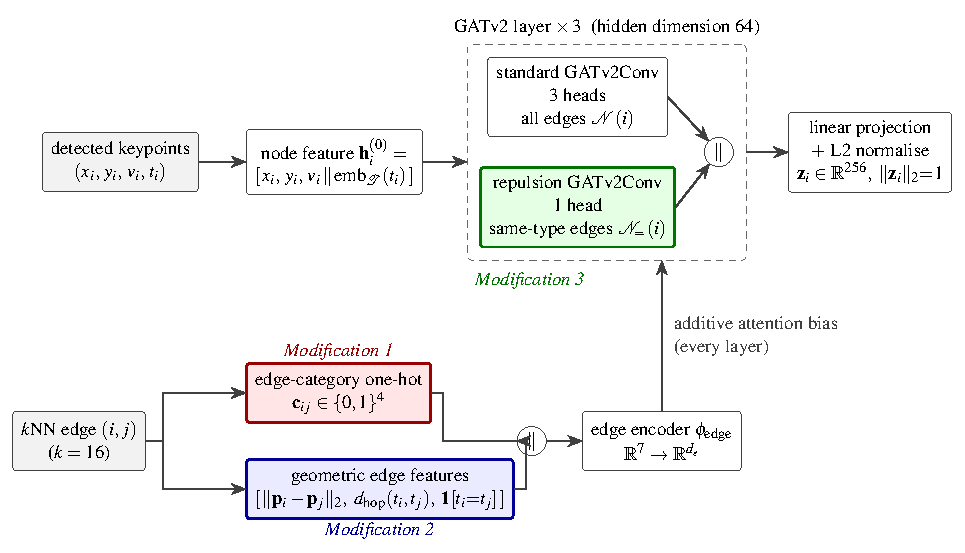
\includegraphics[width=\textwidth]{figures/pggat_architecture.pdf}
    \caption{The PG-GAT layer.
    The node feature contains the keypoint position, the visibility flag and a learned joint-type embedding.
    Modification~1 assigns every edge to one of four categories
    and supplies the one-hot category to the GATv2 attention through a learned additive bias (red).
    Modification~2 adds three geometric features to the edge representation: the Euclidean distance, the skeleton hop distance
    and a same-type indicator (blue).
    Modification~3 splits the multi-head attention into a standard sub-layer over the full neighbourhood
    and a repulsion sub-layer restricted to same-type edges (green).}
    \label{fig:pggat}
\end{figure*}

\paragraph{Modification 1: type-pair attention bias}
Every edge $(i,j) \in \mathcal{E}$ is assigned to one of four mutually exclusive categories according to the joint
types $(t_i,t_j)$ (Figure~\ref{fig:edges}).
\textsc{Same-Type} edges join two detections of the same joint type, which cannot belong to the same skeleton;
\textsc{Skeletal-Neighbour} edges join joint types directly connected in the skeleton, such as a shoulder
and an elbow;
\textsc{Same-Limb} edges join joint types on the same anatomical chain that are not directly connected,
such as a shoulder and a wrist;
\textsc{Cross-Body} covers all remaining pairs.
The skeleton used for these categories has sixteen edges: the head joints (nose, eyes,
ears) are connected among themselves but not to the shoulders, and head-body pairs fall in the cross-body
category.
The category is encoded as a one-hot vector $\mathbf{c}_{ij}\in\{0,1\}^{4}$
and passed through a small edge encoder $\phi_{\text{edge}}$,
\begin{equation}
    \mathbf{e}_{ij}^{\text{cat}}
    =
    \phi_{\text{edge}}(\mathbf{c}_{ij})
    \in \mathbb{R}^{d_e}.
    \label{eq:edge_cat}
\end{equation}
The resulting feature enters the GATv2 attention as an edge feature~\citep{fey2019pyg},
adding a learned edge-dependent term to the attention pre-activation,
\begin{equation}
    \alpha_{ij}^{(l)}
    \propto
    \exp\!\Bigl(
        \mathbf{a}^{(l)\top}
        \mathrm{LeakyReLU}\!\bigl(
            \mathbf{W}^{(l)}
            [\,\mathbf{h}_i^{(l)} \,\|\, \mathbf{h}_j^{(l)}\,]
            +
            \mathbf{W}_e^{(l)}
            \mathbf{e}_{ij}^{\text{cat}}
        \bigr)
    \Bigr),
    \label{eq:pggat_typeattn}
\end{equation}
where $\mathbf{a}^{(l)}$, $\mathbf{W}^{(l)}$ and $\mathbf{W}_e^{(l)}$ are learned parameters of layer $l$.
The four categories therefore receive their own learned responses,
rather than their significance having to be inferred from the node features alone.
An earlier implementation, in which a custom scatter-based attention gave each category its own projection parameters,
was numerically unstable and was replaced by this formulation.

\begin{figure}[!t]
    \centering
    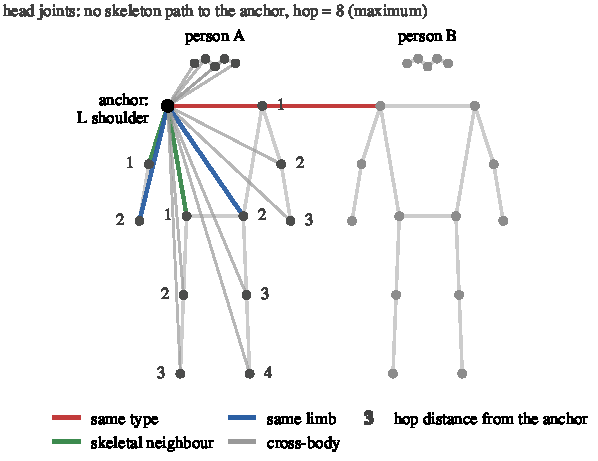
\includegraphics[width=\columnwidth]{figures/edge_categories.pdf}
    \caption{The four edge categories and the skeleton hop distance, drawn from one anchor joint.
    Every edge from the left shoulder of person A is coloured by its category, with the same-type edge
    running to the left shoulder of person B.
    The numbers give the hop distance from the anchor on the sixteen-edge skeleton;
    the head joints have no path to the anchor and take the maximum value.}
    \label{fig:edges}
\end{figure}

\paragraph{Modification 2: skeleton-relative position encoding}
In the baseline, position reaches the attention only through the node features,
and the relative geometry between two connected keypoints must therefore be inferred from the two endpoint representations.
The second modification supplies that geometry directly, adding three features to each edge:
the Euclidean distance $\|\mathbf{p}_i-\mathbf{p}_j\|_2$, the skeleton hop distance $d_{\text{hop}}(t_i,t_j)$
--- the shortest-path distance between the joint types on the skeleton, normalised to $[0,1]$ ---
and a same-type indicator $\mathbb{1}[t_i=t_j]$.
These are concatenated with the category encoding to form the edge descriptor
\begin{equation}
    \mathbf{g}_{ij}
    =
    \left[
        \mathbf{c}_{ij}
        \,\middle\|\,
        \|\mathbf{p}_i-\mathbf{p}_j\|_2
        \,\middle\|\,
        d_{\text{hop}}(t_i,t_j)
        \,\middle\|\,
        \mathbb{1}[t_i=t_j]
    \right]
    \in \mathbb{R}^{7},
    \label{eq:edge_descriptor}
\end{equation}
which passes through the same edge encoder, $\mathbf{e}_{ij}^{\text{geom}} = \phi_{\text{edge}}(\mathbf{g}_{ij})$,
and enters the attention in the same way as Equation~\eqref{eq:pggat_typeattn}.
The hop distance is the most direct description of anatomical structure:
a shoulder and an elbow are one hop apart, a shoulder and an ankle several,
and equal proximity in the image does not carry equal grouping evidence.

\paragraph{Modification 3: same-type repulsion heads}
In a standard layer with $H$ heads, every head attends over the same neighbourhood,
and the signal that separates two left-elbow detections is learned by heads that also model anatomically different
joints.
The third modification reserves capacity for this case.
The layer is split into a standard GATv2 sub-layer with $H_{\text{std}}$ heads over the full neighbourhood $\mathcal{N}(i)$
and a repulsion sub-layer with $H_{\text{rep}}$ heads restricted to same-type edges,
\begin{equation}
    \mathcal{N}_{=}(i)
    =
    \{j \in \mathcal{N}(i) : t_j=t_i\},
    \label{eq:same_type_nbhd}
\end{equation}
with $H_{\text{std}}+H_{\text{rep}}=H$.
The two outputs are concatenated along the head dimension,
\begin{align}
    \mathbf{h}_i^{(l+1)}
    =
    \bigl[\,
        &\mathrm{GATv2Conv}_{\text{std}}
        (\mathbf{h}^{(l)},\mathcal{N}(i))
        \,\big\|\, \nonumber \\
        &\mathrm{GATv2Conv}_{\text{rep}}
        (\mathbf{h}^{(l)},\mathcal{N}_{=}(i))
    \,\bigr],
    \label{eq:pggat_repulsion}
\end{align}
leaving the head count of the layer unchanged.
The repulsion heads see only the comparisons that decide between people of the same joint type,
and the final configuration assigns one of the four heads to this pathway, $H_{\text{rep}}=1$ and $H_{\text{std}}=3$.

\paragraph{Network}
The final PG-GAT has three such layers with four heads and a hidden dimension of 64,
each followed by layer normalisation, a nonlinearity and dropout of 0.1.
A linear projection maps the final representation to the embedding $\mathbf{z}_i \in \mathbb{R}^{256}$,
which is L2-normalised so that every embedding lies on the unit hypersphere.
This bounds the space in which the read-out operates and makes the inner product of two embeddings equal to their cosine
similarity.
These settings were selected by an architecture search rather than inherited from the baseline.

\subsection{Training}
\label{sec:method_training}

% --- from chapter3_baseline.tex 3.5.2-3.5.3 and chapter3_pg_gat.tex 3.8.5 ---
The embedding network is trained with a margin-based contrastive loss~\citep{chopra2005contrastive} on cosine similarity,
$\cos(\mathbf{z}_i,\mathbf{z}_j) = \mathbf{z}_i^\top \mathbf{z}_j$.
Positive pairs $\mathcal{P}^{+}$ contain keypoints of the same person,
$\mathbf{y}^\star_i = \mathbf{y}^\star_j$ with $i \neq j$;
negative pairs $\mathcal{P}^{-}$ contain keypoints of different people.
The objective is
\begin{align}
    \mathcal{L}_{\text{contrastive}}
    =
    &\frac{1}{|\mathcal{P}^{+}|}
    \sum_{(i,j) \in \mathcal{P}^{+}}
    \bigl(
        1 - \cos(\mathbf{z}_i,\mathbf{z}_j)
    \bigr) \nonumber \\
    &+\;
    \frac{1}{|\mathcal{P}^{-}|}
    \sum_{(i,j) \in \mathcal{P}^{-}}
    \max\!\bigl(
        0,\;
        \cos(\mathbf{z}_i,\mathbf{z}_j) - \gamma
    \bigr).
    \label{eq:contrastive_loss}
\end{align}
The first term pulls same-person embeddings towards a cosine similarity of one
and keeps contributing however close they already are.
The second term penalises different-person pairs whose similarity exceeds the margin $\gamma$;
once a negative pair falls below the margin it no longer contributes,
which keeps the gradient on the pairs that are still too close.
The margin is set to $\gamma=0.5$.
For the repulsion heads of Section~\ref{sec:method_pggat}, which see only same-type edges,
the second term is the signal that separates same-type detections of different people.

Training proceeds in two stages.
The network is first trained on 400 procedurally generated synthetic scenes with known person identities,
for 50 epochs at a batch size of 4,
using AdamW~\citep{loshchilov2019adamw} at an initial learning rate of $10^{-3}$ and weight decay $10^{-4}$,
cosine annealing~\citep{loshchilov2017cosineannealing} to $10^{-5}$,
and gradient-norm clipping at 1.0.
The checkpoint with the highest pose grouping accuracy on a held-out synthetic validation split is kept.
It is then fine-tuned on the person-keypoint annotations of COCO \texttt{train2017}~\citep{lin2014coco} under the same
objective, for a smaller number of epochs at a reduced learning rate,
to adapt the embedding to real keypoint statistics while retaining the person-separation structure learned on synthetic
data.
Synthetic pre-training provides exact identities, controlled scene composition and a repeatable setting in
which design changes can be compared without the variation a real detector introduces;
the fine-tuning stage closes the gap to real data.

Apart from the neighbourhood size $k$, the principal hyperparameters of the final model were selected by search rather
than inherited.
Six architectural parameters (number of layers, number of heads, hidden dimension, output dimension,
joint-type embedding dimension and dropout) were selected by a 32-run Bayesian sweep with Hyperband early
termination~\citep{li2018hyperband}, with pose grouping accuracy on the synthetic validation split as the selection
metric; the sweep settled on the three-layer, four-head,
256-dimensional configuration above.
A separate 24-run sweep over the contrastive margin, the number of repulsion heads, the learning rate
and the weight decay returned settings close to the inherited ones, including $\gamma=0.5$,
and the improvement of PG-GAT over the baseline is therefore not a product of retuning the objective.
A further 12-run sweep over the fine-tuning epochs, learning rate and weight decay,
centred on a 20-epoch recipe at $10^{-4}$, selected the 15-epoch schedule.

\subsection{Read-out and person count}
\label{sec:method_readout}

% --- from chapter3_baseline.tex 3.5.3 (read-out) and chapter3_integration.tex 3.12.4 (K estimation), brief per D5 ---
At inference the network is applied once per image to produce the embeddings $\{\mathbf{z}_i\}_{i=1}^{N}$,
which are grouped by $k$-means with $K$ clusters on the unit hypersphere, using ten random initialisations
and a fixed seed~\citep{scikitlearn}.
The read-out is unchanged from the baseline and applies no structural constraint;
PG-GAT changes the representation on which grouping is performed, not the clustering.

When no oracle count is available, $K$ is predicted by a small head, the K-head, trained on the frozen embeddings.
The node embeddings of a scene are summarised by concatenating their mean-pooled
and max-pooled representations with the keypoint count normalised by the seventeen joint types;
a multilayer perceptron maps this vector to a person count and is trained with an L1 loss against the ground-truth
$K$.
Training the head jointly with the embedding network lets the count gradient reach the embedding
and degrades its person separation; the head is therefore trained after the embedding network,
with all embedding parameters frozen.
The final K-head has 35\,009 parameters.
Because keypoint visibility, missing detections and person density differ between synthetic and real data,
the K-head used on COCO is trained on embeddings of COCO \texttt{train2017} scenes, again with PG-GAT frozen.
Two settings are evaluated: oracle $K$, which measures the embedding and read-out alone,
and predicted $\hat K$, which is the complete autonomous pipeline.